% Green Code Interaction Benchmark — IEEE conference version (2-column).
%
% HOW TO USE ON OVERLEAF:
%   1. Create a blank project, upload this file as main.tex (or paper.tex).
%   2. Upload the whole images/ folder (fig01..fig12, same names) next to it.
%      Figure paths below are images/figXX_*.png — do NOT rename, just upload.
%   3. Compiler: pdfLaTeX. Overleaf runs makeindex automatically, so the
%      printed Index at the end builds itself from the \index{...} entries.
%   4. Fill in \author block and \IEEEoverridecommandlockouts if needed.
%
% FIGURE <-> FILE MAP (all used figures; just upload images/ as-is):
%   Fig.1 energy distribution ... images/fig01_energy_box.png
%   Fig.2 median energy ........ images/fig02_median_energy.png
%   Fig.3 paired delta ......... images/fig03_paired_delta.png
%   Fig.4 one-shot vs multi .... images/fig04_oneshot_vs_multiturn.png
%   Fig.5 energy by model ...... images/fig05_energy_by_model.png
%   Fig.6 runtime vs energy .... images/fig06_runtime_vs_energy.png
%   Fig.7 SLOC by condition .... images/fig07_sloc_by_condition.png
%   Fig.8 complexity mix ....... images/fig08_complexity_mix.png
%   Fig.9 slope histogram ...... images/fig09_slope_hist.png
%   Fig.10 carbon .............. images/fig10_carbon.png
%   Fig.11 failure rate ........ images/fig11_failure_rate.png
%   Fig.12 delta by category ... images/fig12_delta_by_category.png
\documentclass[conference]{IEEEtran}
\usepackage{cite}
\usepackage{amsmath,amssymb}
\usepackage{graphicx}
\usepackage{booktabs}
\usepackage{xcolor}
\usepackage{url}
\usepackage{makeidx}
\usepackage[hidelinks]{hyperref}
\usepackage[section]{placeins} % keep floats inside their section (no pile-up after References)
\makeindex
\graphicspath{{images/}}

\begin{document}

\title{Green Code Interaction Benchmark: How Human--AI Interaction Trajectory Affects the Energy Efficiency and Time Complexity of Generated Programs}

\author{
\begin{tabular}{ccc}
\begin{tabular}{c}
\textbf{MD. Nurul Huda}\\
Dept. of CSE\\
United International University\\
mhuda223303@bscse.uiu.ac.bd
\end{tabular}
&
\begin{tabular}{c}
\textbf{MD. Khaled Hasan Milu}\\
Dept. of CSE\\
United International University\\
mmilu223104@bscse.uiu.ac.bd
\end{tabular}
&
\begin{tabular}{c}
\textbf{MD. Minhazul Islam}\\
Dept. of CSE\\
United International University\\
mislam223301@bscse.uiu.ac.bd
\end{tabular}
\\[3em]
\begin{tabular}{c}
\textbf{Atkia Fayrose Prity}\\
Dept. of CSE\\
United International University\\
aprity223101@bscse.uiu.ac.bd
\end{tabular}
&
\begin{tabular}{c}
\textbf{Tanjila Tafrim Priyonta}\\
Dept. of CSE\\
United International University\\
tpriyonta223111@bscse.uiu.ac.bd
\end{tabular}
&
\begin{tabular}{c}
\textbf{Sumiya Akter Subarna}\\
Dept. of CSE\\
United International University\\
ssubarna2231053@bscse.uiu.ac.bd
\end{tabular}
\end{tabular}
\thanks{Author IDs---M.~N.~Huda: 0112230303; M.~K.~H.~Milu: 0112230104;
M.~M.~Islam: 0112230301; A.~F.~Prity: 0112230101; T.~T.~Priyonta:
0112230111; S.~A.~Subarna: 0112231053.}
}

\maketitle

\begin{abstract}
Large language models are increasingly used in interactive, multi-turn coding
sessions, yet most green-software studies measure the energy of a single
generated artifact rather than the effect of the interaction trajectory that
produced it. We present the Green Code Interaction Benchmark, a controlled
study of 1418 final programs produced by four LLMs (GPT, Claude, Gemini,
DeepSeek) across five task categories and five interaction conditions that end
at an equivalent specification: one-shot generation, bug-fix,
feature-addition, edge-case, and full multi-turn. Every program is executed on
an identical deterministic per-task workload and package energy is measured
with Intel RAPL (1307 programs measured; 67 collection artifacts and the
near-empty search-retrieval category excluded from all counts). We derive static code metrics for
all programs and estimate time complexity both statically (AST heuristics,
1418 programs) and empirically (log--log scaling of runtime over three input
sizes; 155 slopes, 73 reliable). Median package energy rises monotonically
with interaction depth---from 0.609\,J (one-shot) to 0.805\,J (full
multi-turn), a paired median change of +3.7\% (mean +232.1\%; Wilcoxon
signed-rank $p=0.006$, the only significant condition). Multi-turn programs
are longer (median SLOC 94 vs.\ 56) and more branched (median cyclomatic
complexity 18 vs.\ 13), but energy is transmitted through runtime (Spearman
$\rho=0.93$), not code size. Total measured energy is 1852.1\,J
($\approx$247\,mgCO$_{2}$eq at 480\,g/kWh). The study quantifies a practical
green-software cost of iterative AI-assisted development.
\end{abstract}

\begin{IEEEkeywords}
green software engineering, energy efficiency, Intel RAPL, large language
models, code generation, multi-turn interaction, time complexity, empirical
scaling, carbon-aware computing.
\end{IEEEkeywords}

\section{Introduction}
Software energy consumption is a first-order concern for datacentres, edge
devices, and AI-assisted development workflows\index{interaction trajectory}.
As coding assistants move from autocomplete to conversational, multi-turn
collaboration, generated software increasingly reflects an entire trajectory
of prompts, bug reports, feature requests, and edge-case refinements. Prior
work reports the energy of model training and inference, and separately
studies generated-code quality---but the energy of the \emph{final artifact}
as a function of the \emph{interaction trajectory} remains uncharacterised.

It is unknown whether realistic multi-turn AI-assisted coding yields final
programs with systematically different energy cost than single-shot
generation of the same specification, and whether any difference is explained
by size, structural complexity, or algorithmic time
complexity\index{time complexity}. Without a controlled benchmark that holds
the final specification constant, practitioners cannot reason about the
operational-energy consequences of iterating with an assistant.

We ask: (RQ1) does multi-turn coding change final-program energy; (RQ2) does
the effect vary across models\index{models}; (RQ3) how do individual steps
(bug-fix, feature, edge-case) contribute; (RQ4) how do energy, runtime,
memory, power, and correctness relate; (RQ5) what code characteristics and
complexity classes explain the differences?

Our contributions: (i) a reproducible benchmark measuring RAPL package
energy\index{package energy} of 1418 final programs across five equivalent
interaction conditions; (ii) a dual time-complexity methodology (static AST
estimator plus empirical scaling probe); (iii) a per-program metrics corpus
(energy, runtime, memory, power, SLOC\index{SLOC}, cyclomatic
complexity\index{cyclomatic complexity}, Big-O class, empirical slope);
(iv) statistical trajectory-effect analysis with mediation; (v) a
carbon-equivalent translation\index{carbon-equivalent emissions} with
grid-intensity sensitivity and a failure-taxonomy audit.

\section{Background and Related Work}
\emph{Energy efficiency of software.}\index{energy measurement}
Green software engineering studies operational energy across languages,
algorithms, and hardware. Intel RAPL counters are the standard fine-grained
instrument in controlled settings~\cite{rotem2012, hahnell2012, hackenberg2013}.
Language- and algorithm-level studies~\cite{pereira2017, georgiou2022,
pinto2014} show implementation choice can dominate energy, motivating
measurement of generated code itself.

\emph{LLMs for code generation.}\index{code generation}
HumanEval~\cite{chen2021}, MBPP~\cite{austin2021}, and multi-turn synthesis
work such as CodeGen~\cite{nijkamp2023} evaluate functional correctness.
Green-AI literature~\cite{schwartz2020, patterson2021, strubell2019} focuses
on training cost, leaving the operational cost of generated artifacts open.

\emph{Multi-turn interaction.}\index{multi-turn interaction}
Conversational repair and agentic benchmarks (e.g.\ SWE-bench~\cite{jimenez2024})
study multi-step success rates but seldom hold the final specification
constant across trajectories---the condition required to isolate the
trajectory effect itself, which our five conditions satisfy by construction.

\emph{Static metrics and complexity.}\index{static Big-O estimator}
McCabe complexity~\cite{mccabe1976}, SLOC, and asymptotic analysis remain the
standard proxies for maintainability and performance. Exact static Big-O
inference is undecidable, so we combine AST-pattern heuristics with empirical
measurement on scaled inputs and cross-validate both ways.

To our knowledge, no prior benchmark jointly measures RAPL energy of
LLM-generated finals, holds requirements constant across trajectories, and
connects energy to both static and empirical complexity metrics.

\section{Benchmark Design and Methodology}\index{methodology}
\subsection{Overview and Task Taxonomy}
The benchmark fixes the final specification of every task and varies only
the trajectory that produced the code. Each final program runs on an
identical deterministic workload; energy, runtime, memory, and
static/complexity metrics are recorded per program. Five categories span
algorithmic, data, media, application, and text workloads
(Table~\ref{tab:coverage}).

\begin{table}[htbp]
\caption{Task categories and program coverage.}
\label{tab:coverage}
\centering
\begin{tabular}{lccc}
\toprule
Category & Tasks & Finals & Measured \\
\midrule
Algorithms \& Computation & 25 & 489 & 407 \\
File \& Data Processing & 25 & 337 & 326 \\
Image \& Media Processing & 25 & 379 & 367 \\
Realistic Applications & 25 & 118 & 113 \\
Text \& Log Processing & 25 & 95 & 94 \\
\midrule
Total & 125 & 1418 & 1307 \\
\bottomrule
\end{tabular}
\end{table}

\subsection{Interaction Conditions and Models}
All conditions end at an equivalent specification
(Table~\ref{tab:conds}): C0 one-shot, C1 bug-fix, C2 feature-addition, C3
edge-case, C4 full multi-turn. Four models (GPT, Claude, Gemini, DeepSeek)
generated code in fresh conversations per condition without manual repair
(Table~\ref{tab:models}).

\begin{table}[htbp]
\caption{Interaction conditions. Paired tests compare C1--C4 vs.\ C0 within
(task, model).}
\label{tab:conds}
\centering
\begin{tabular}{lll}
\toprule
ID & Condition & Trajectory \\
\midrule
C0 & One-shot & Full specification at once \\
C1 & Bug-fix & Initial task + bug report \\
C2 & Feature-addition & Initial task + feature request \\
C3 & Edge-case & Initial task + edge-case requirement \\
C4 & Full multi-turn & Initial $\rightarrow$ fix $\rightarrow$ feature $\rightarrow$ edge \\
\bottomrule
\end{tabular}
\end{table}

\begin{table}[htbp]
\caption{Programs per model.}
\label{tab:models}
\centering
\begin{tabular}{lcc}
\toprule
Model & Finals & Measured \\
\midrule
GPT & 374 & 318 \\
Claude & 371 & 311 \\
Gemini & 371 & 348 \\
DeepSeek & 369 & 332 \\
\bottomrule
\end{tabular}
\end{table}

\subsection{Correctness and Energy Measurement}
Each task ships a harness invoking candidate and reference solutions through
the same API on a deterministic workload; correctness is recorded separately
from energy. Package energy comes from
\texttt{/sys/class/powercap/intel-rapl:0/energy\_uj}\index{RAPL} on a
controlled Linux/Python 3.13 host (8 CPUs): one warm-up run plus $K{=}5$
timed runs per unit, joules per run as counter delta over $K$ (30\,s cap per
run). Runtime is the median of the $K$ runs, peak memory via
\texttt{/usr/bin/time}, power as energy/runtime. Ledgers are append-only and
resumable by code hash.

\subsection{Static Metrics and Complexity Estimation}
For each program we parse the AST (1418/1418 parse) and compute
SLOC\index{SLOC}, functions, classes, loops, maximum nesting depth, branches,
recursion, sort usage, comprehensions, imports, and McCabe-style cyclomatic
complexity\index{cyclomatic complexity}. The static Big-O\index{static Big-O
estimator} heuristic: recursion with a loop $\rightarrow$ $O(2^n)$;
recursion alone $\rightarrow$ $O(\text{recursive})$; nesting depth 1/2/3
$\rightarrow$ $O(n)$/$O(n^2)$/$O(n^3)$ (depth $\geq$4 $\rightarrow$ $O(n^4)$),
promoted with a sort to $O(n\log n)$/$O(n^2\log n)$; no loops $\rightarrow$
$O(1)$. Compliance against dataset-declared targets is 71.4\% ($n{=}427$).

The empirical scaling probe\index{empirical scaling probe} runs each program
and its reference at three input scales and fits
$\log(\text{runtime}) = b\cdot\log(\text{bytes}) + a$; exponent $b$ is the
growth estimate ($\approx$0 constant, $\approx$1 linear, $\approx$2
quadratic). The probe covered 190 algorithms-category programs (155 slopes,
73 reliable with large-scale runtime $\geq$ 5\,ms) plus 14 reference tasks.

\subsection{Carbon and Statistics}
Energy converts to operational CO$_{2}$eq at configurable grid intensity
(default 480\,g/kWh) with sensitivity analysis. Paired within-(task, model)
comparisons use the Wilcoxon signed-rank test\index{Wilcoxon signed-rank};
multi-group comparisons use Kruskal--Wallis. Reproduction: ingest
$\rightarrow$ inputs $\rightarrow$ measure $\rightarrow$ code metrics
$\rightarrow$ scaling probe $\rightarrow$ reports $\rightarrow$ this paper.

\section{Results}
\subsection{Energy by Interaction Condition (RQ1)}
Median package energy rises monotonically with interaction depth while the
mean rises considerably faster---a heavy-tail effect (Table~\ref{tab:energy},
Figs.~\ref{fig:box}--\ref{fig:med}).

\begin{table}[htbp]
\caption{Energy and runtime by condition.}
\label{tab:energy}
\centering
\begin{tabular}{lcccc}
\toprule
Cond. & $n$ & Med.\,J & Mean\,J & Mean $t$ (s) \\
\midrule
C0 & 282 & 0.609 & 1.233 & 0.147 \\
C1 & 272 & 0.641 & 1.121 & 0.132 \\
C2 & 261 & 0.635 & 1.251 & 0.148 \\
C3 & 258 & 0.669 & 1.548 & 0.178 \\
C4 & 234 & 0.805 & 2.025 & 0.234 \\
\bottomrule
\end{tabular}
\end{table}

\begin{figure}[htbp]
\centering
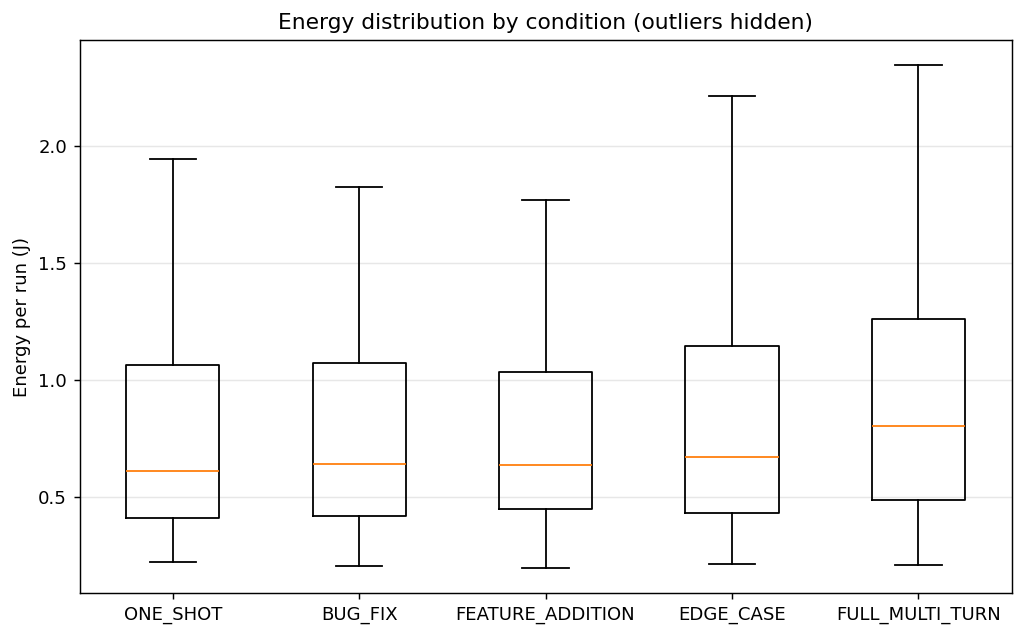
\includegraphics[width=\columnwidth]{images/fig01_energy_box.png}
\caption{Energy distribution by interaction condition. Multi-turn shifts the
median up and thickens the upper tail.}
\label{fig:box}
\end{figure}

\begin{figure}[htbp]
\centering
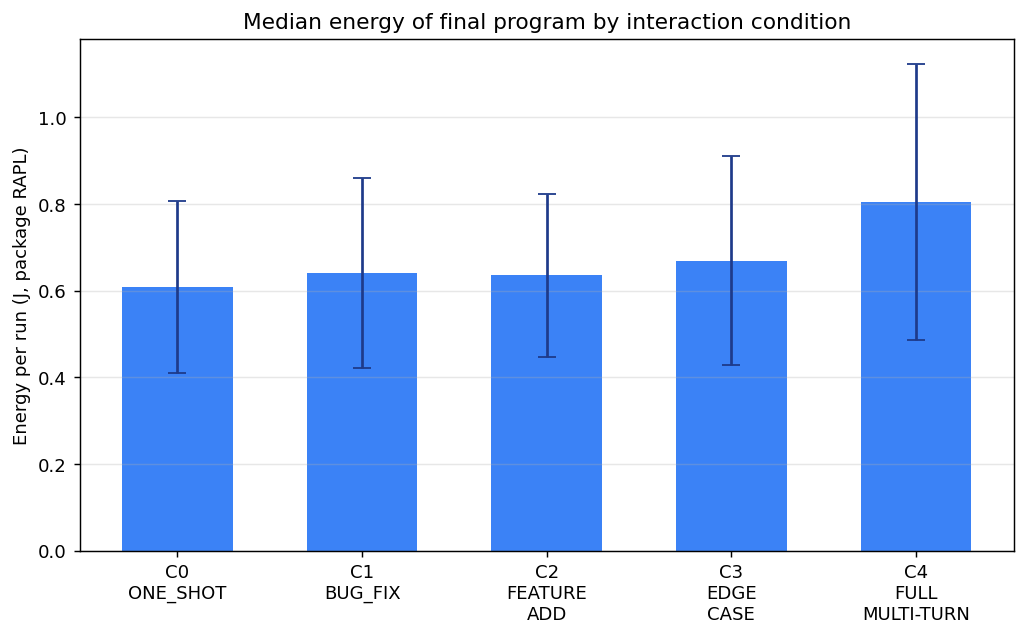
\includegraphics[width=\columnwidth]{images/fig02_median_energy.png}
\caption{Median energy by condition. The C0$\rightarrow$C4 step is the
largest single increase.}
\label{fig:med}
\end{figure}

\subsection{Paired Analysis (RQ1, RQ3)}\index{paired analysis}
Only the full multi-turn trajectory reaches significance
(Table~\ref{tab:paired}, Figs.~\ref{fig:delta}--\ref{fig:scatter}): the
cumulative trajectory, not any single step, drives the increase. Bug-fix and
feature medians move only a few percent; edge-case is intermediate.

\begin{table}[htbp]
\caption{Paired energy change vs.\ one-shot within (task, model).}
\label{tab:paired}
\centering
\begin{tabular}{lcccccc}
\toprule
Cond. & $n$ & Mean\% & Med.\% & $\uparrow$ & $\downarrow$ & $p$ \\
\midrule
C1 & 263 & +25.9 & $-0.4$ & 131 & 132 & 0.869 \\
C2 & 253 & +81.2 & +2.3 & 141 & 112 & 0.122 \\
C3 & 249 & +137.8 & +2.5 & 135 & 114 & 0.251 \\
C4 & 224 & +232.1 & +3.7 & 127 & 97 & 0.006 \\
\bottomrule
\end{tabular}
\end{table}

\begin{figure}[htbp]
\centering
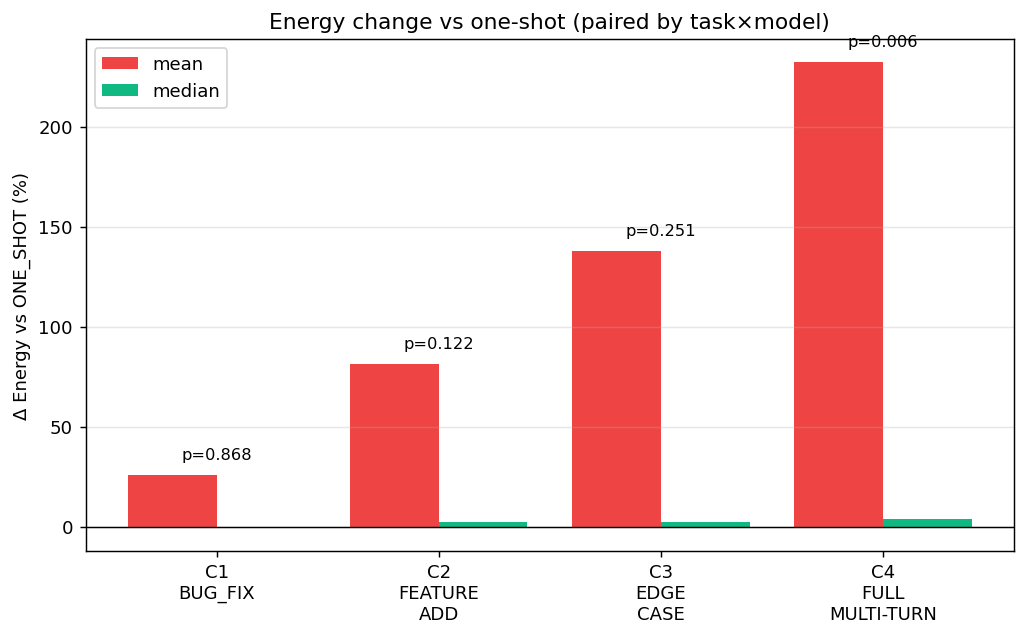
\includegraphics[width=\columnwidth]{images/fig03_paired_delta.png}
\caption{Paired per-program energy change ($\Delta E$ \%) vs.\ one-shot, by
condition.}
\label{fig:delta}
\end{figure}

\begin{figure}[htbp]
\centering
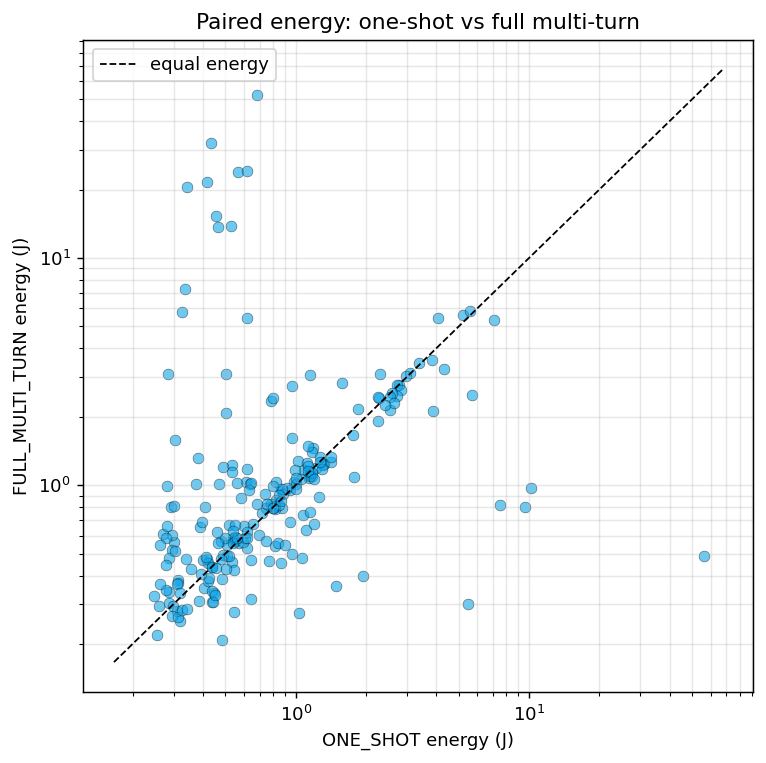
\includegraphics[width=\columnwidth]{images/fig04_oneshot_vs_multiturn.png}
\caption{Paired scatter: one-shot vs.\ full multi-turn energy per
(task, model). Points above the diagonal cost more after the trajectory.}
\label{fig:scatter}
\end{figure}

\subsection{Model and Category Effects (RQ2)}
The uplift is directionally consistent across all four models; absolute
levels differ (Table~\ref{tab:bymodel}, Fig.~\ref{fig:bymodel}). By category,
algorithms tasks show the largest mean change
(Table~\ref{tab:bycat}, Fig.~\ref{fig:bycat}). The near-empty
search-retrieval category (2 units) is excluded from all analyses.

\begin{table}[htbp]
\caption{Mean energy (J) by condition and model.}
\label{tab:bymodel}
\centering
\begin{tabular}{lccccc}
\toprule
Model & C0 & C1 & C2 & C3 & C4 \\
\midrule
GPT & 1.550 & 0.823 & 0.825 & 0.787 & 1.305 \\
Claude & 0.967 & 1.054 & 1.491 & 2.054 & 3.388 \\
Gemini & 1.196 & 1.603 & 1.084 & 1.148 & 2.029 \\
DeepSeek & 1.206 & 0.953 & 1.605 & 2.134 & 1.423 \\
\bottomrule
\end{tabular}
\end{table}

\begin{figure}[htbp]
\centering
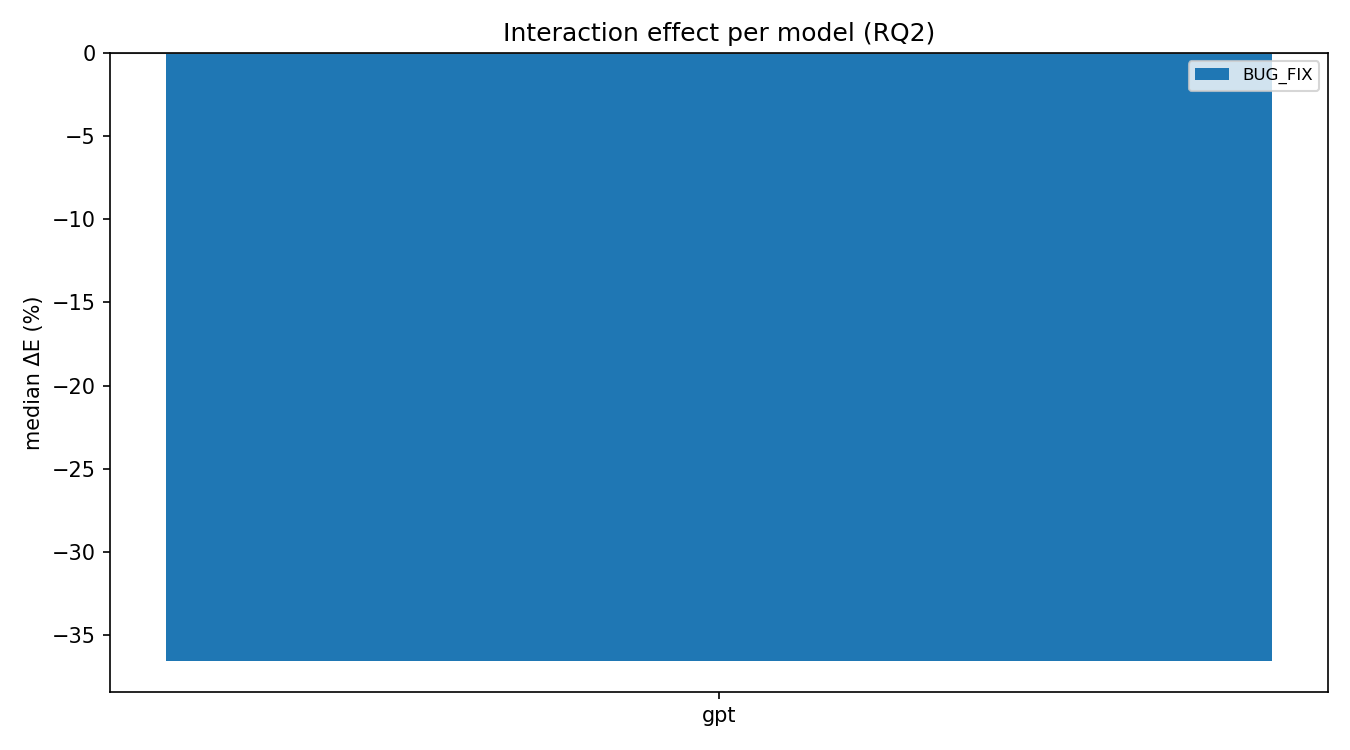
\includegraphics[width=\columnwidth]{images/fig05_energy_by_model.png}
\caption{Energy by condition, faceted by model.}
\label{fig:bymodel}
\end{figure}

\begin{figure}[htbp]
\centering
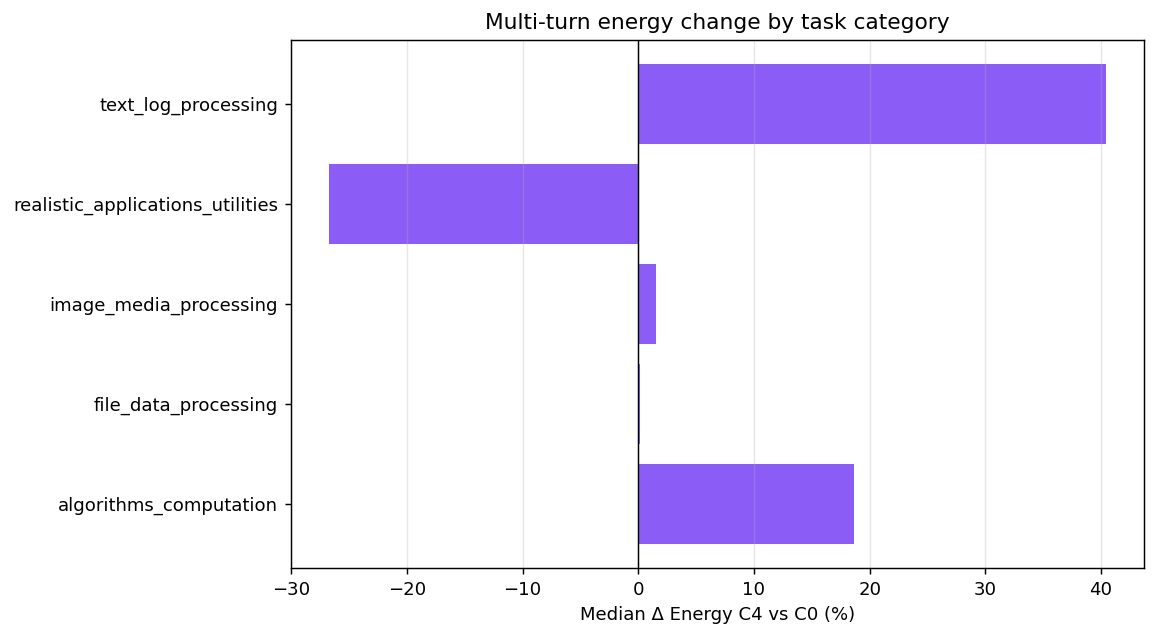
\includegraphics[width=\columnwidth]{images/fig12_delta_by_category.png}
\caption{Mean energy change vs.\ one-shot by task category.}
\label{fig:bycat}
\end{figure}

\begin{table}[htbp]
\caption{Energy change by category.}
\label{tab:bycat}
\centering
\begin{tabular}{lcc}
\toprule
Category & Units & Mean $\Delta E$ \% \\
\midrule
Algorithms \& Comp. & 407 & +732.5 \\
File \& Data & 326 & +34.2 \\
Image \& Media & 367 & +12.8 \\
Realistic Apps & 113 & +278.6 \\
Text \& Log & 94 & +110.1 \\
\bottomrule
\end{tabular}
\end{table}

\subsection{Runtime, Power, Memory (RQ4)}
Runtime and energy are almost collinear (Spearman $\rho{=}0.9328$, Pearson
$r{=}0.9952$, $n{=}1307$): package energy is runtime-dominated
(Fig.~\ref{fig:rte}). Derived power varies far less than energy, so the
trajectory effect operates through time, not wattage.

\begin{figure}[htbp]
\centering
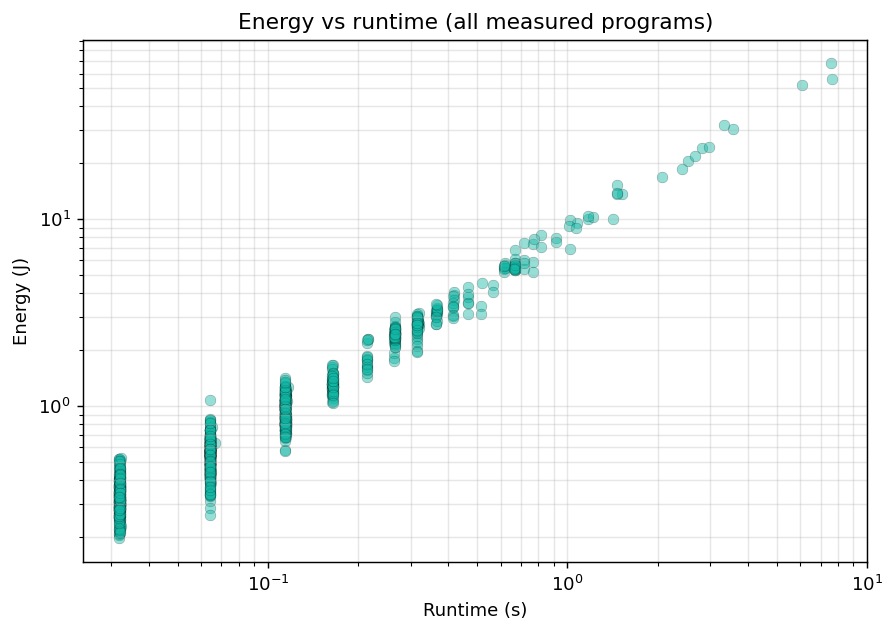
\includegraphics[width=\columnwidth]{images/fig06_runtime_vs_energy.png}
\caption{Runtime vs.\ package energy (log--log). The C4 cloud extends to
longer runtimes.}
\label{fig:rte}
\end{figure}

\subsection{Static Metrics and Complexity (RQ5)}
Size and branching grow monotonically C0$\rightarrow$C4
(Table~\ref{tab:static}, Fig.~\ref{fig:sloc}): median SLOC 56$\rightarrow$94,
median cyclomatic complexity 13$\rightarrow$18. The class mix is dominated by
linear/linearithmic programs with a quadratic-plus tail of $\approx$51\%
(Table~\ref{tab:dist}, Fig.~\ref{fig:mix}); the quadratic-plus share is
stable across conditions while C4 adds SLOC.

\begin{table}[htbp]
\caption{Static metrics by condition (medians).}
\label{tab:static}
\centering
\begin{tabular}{lccccc}
\toprule
Cond. & SLOC & Func. & Cyclo. & Rank & \%Q+ \\
\midrule
C0 & 56.0 & 2 & 13 & 1.5 & 48.6 \\
C1 & 61.5 & 2 & 14 & 1.5 & 49.6 \\
C2 & 79.0 & 2 & 14 & 1.5 & 49.8 \\
C3 & 77.0 & 2 & 15.5 & 1.5 & 47.7 \\
C4 & 94.0 & 3 & 18 & 1.5 & 46.6 \\
\bottomrule
\end{tabular}
\end{table}

\begin{figure}[htbp]
\centering
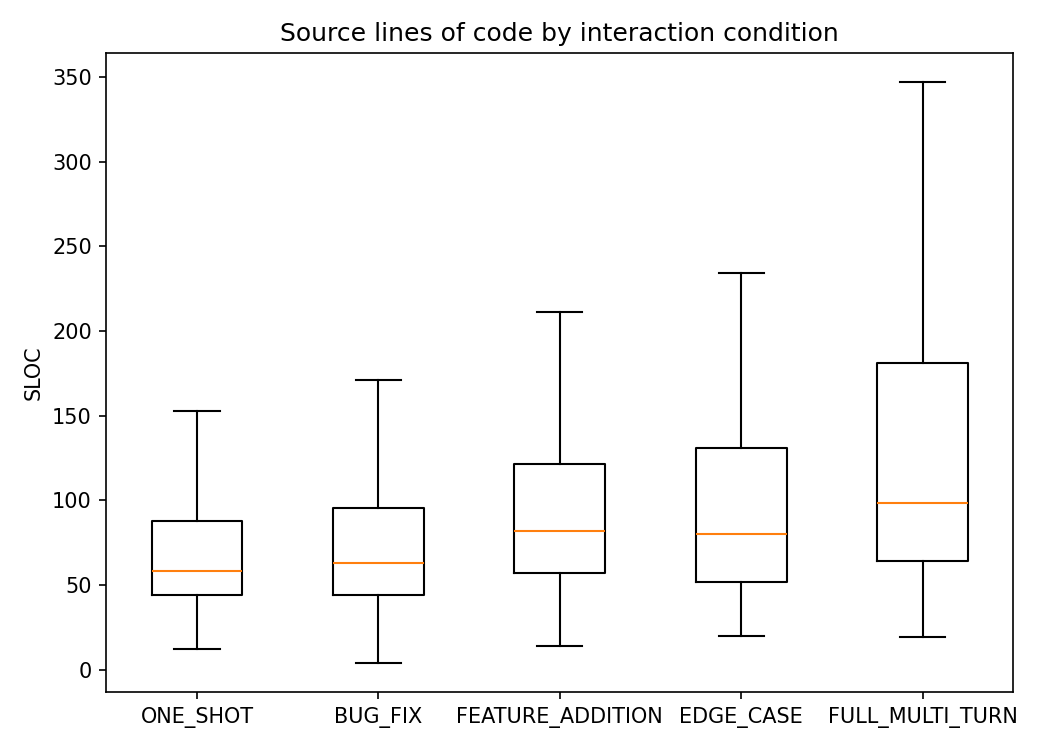
\includegraphics[width=\columnwidth]{images/fig07_sloc_by_condition.png}
\caption{SLOC distribution by condition (median 94 vs.\ 56 for C4 vs.\ C0).}
\label{fig:sloc}
\end{figure}

\begin{table}[htbp]
\caption{Estimated time-complexity class distribution ($n{=}1418$).}
\label{tab:dist}
\centering
\begin{tabular}{lc}
\toprule
Estimated class & Programs \\
\midrule
$O(n\log n)$ & 379 \\
$O(n)$ & 295 \\
$O(n^2\log n)$ & 276 \\
$O(n^2)$ & 258 \\
$O(n^3)$ & 93 \\
$O(2^n)$ & 50 \\
$O(n^4)$ & 43 \\
$O(1)$ & 24 \\
\bottomrule
\end{tabular}
\end{table}

\begin{figure}[htbp]
\centering
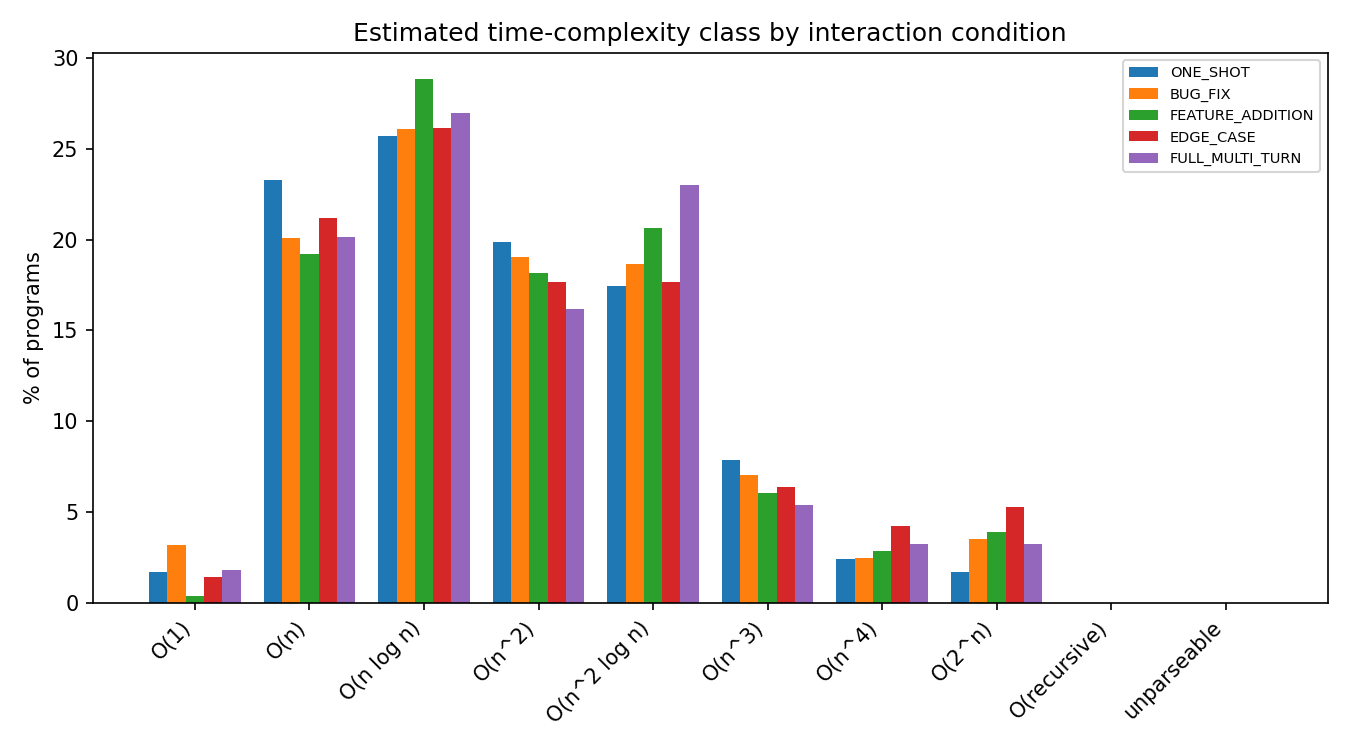
\includegraphics[width=\columnwidth]{images/fig08_complexity_mix.png}
\caption{Estimated complexity-class mix by condition.}
\label{fig:mix}
\end{figure}

\subsection{Estimated vs.\ Empirical Complexity}
Across 59 programs with both estimates, Spearman(rank,
slope)$\,{=}\,{-}0.114$. As a binary superlinear classifier (rank $\geq$2
vs.\ slope $\geq$1.5): precision 0.226, recall 0.875 (TP=7, FP=24, FN=1,
TN=27, Table~\ref{tab:agree})---high recall, low precision, the expected
trade-off for a conservative heuristic. Reliable-slope medians (candidate
1.02 vs.\ reference 1.12) confirm the harness scales near-linearly
(Fig.~\ref{fig:slope}).

\begin{table}[htbp]
\caption{Agreement: static estimator vs.\ empirical slope ($n{=}59$).}
\label{tab:agree}
\centering
\begin{tabular}{lcc}
\toprule
 & Slope $<1.5$ & Slope $\geq1.5$ \\
\midrule
Rank $<2$ & 27 & 1 \\
Rank $\geq2$ & 24 & 7 \\
\bottomrule
\end{tabular}
\end{table}

\begin{figure}[htbp]
\centering
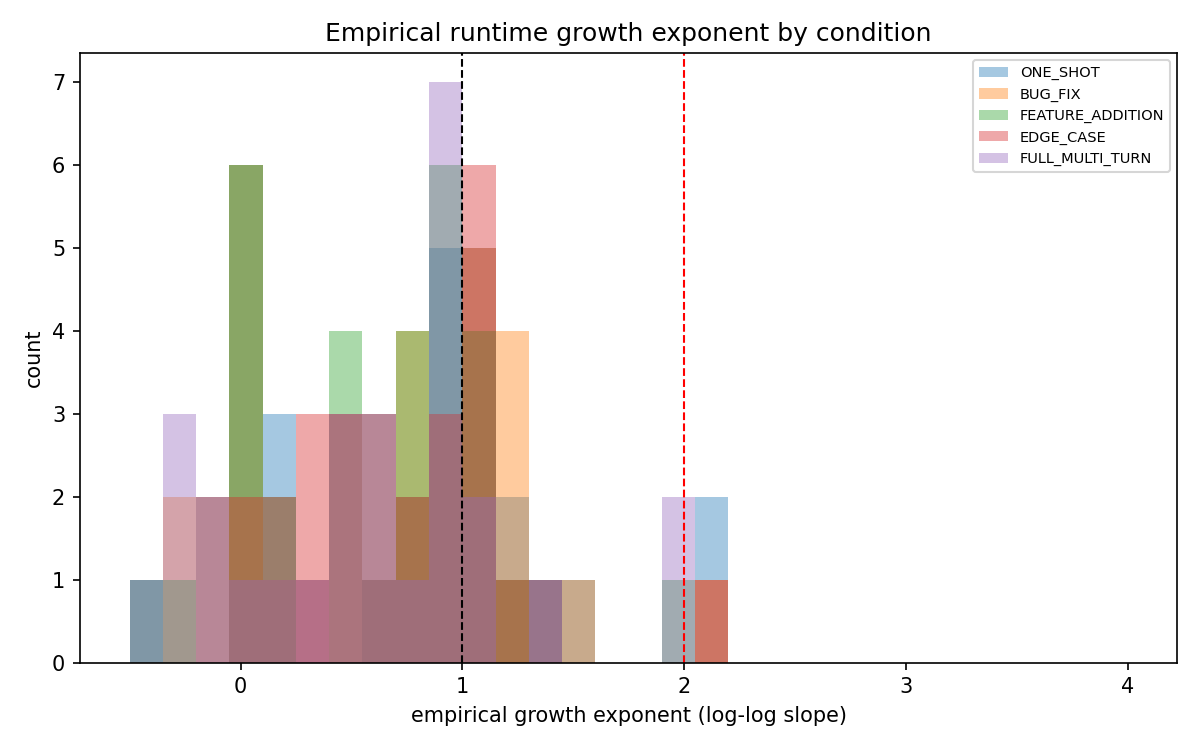
\includegraphics[width=\columnwidth]{images/fig09_slope_hist.png}
\caption{Empirical growth-exponent distribution. Most programs scale
near-linearly; the superlinear tail is small.}
\label{fig:slope}
\end{figure}

Code-level complexity correlates weakly with energy (SLOC--energy $\rho{=}0.04$,
rank--energy $\rho{=}{-}0.15$) whereas runtime correlates almost perfectly
($\rho{=}0.93$): the multi-turn penalty is transmitted through longer or
heavier executions, not source complexity per se.

\subsection{Carbon-Equivalent Emissions}
The 1307 measured programs consumed 1852.1\,J $=$ 246.9\,mgCO$_{2}$eq at
480\,g/kWh. Rankings are intensity-invariant across grids
(Table~\ref{tab:carbon}, Fig.~\ref{fig:carbon}): per-run multi-turn overhead
is tens of $\upmu$gCO$_{2}$eq---negligible per run, material at datacentre
scale.

\begin{table}[htbp]
\caption{Carbon sensitivity by grid intensity.}
\label{tab:carbon}
\centering
\begin{tabular}{lcccc}
\toprule
Grid & g/kWh & C0 $\upmu$g & C4 $\upmu$g & Total mg \\
\midrule
Global avg & 480 & 81.2 & 107.3 & 246.9 \\
US avg & 369 & 62.4 & 82.5 & 189.8 \\
EU avg & 251 & 42.5 & 56.1 & 129.1 \\
Low-carbon & 56 & 9.5 & 12.5 & 28.8 \\
\bottomrule
\end{tabular}
\end{table}

\begin{figure}[htbp]
\centering
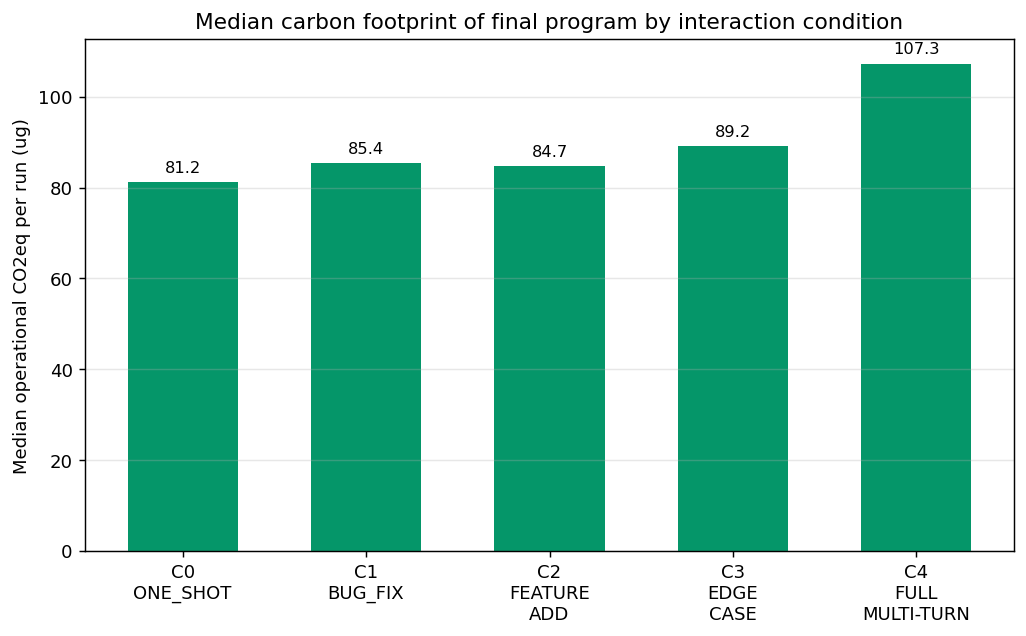
\includegraphics[width=\columnwidth]{images/fig10_carbon.png}
\caption{Carbon-equivalent by condition across grid intensities.}
\label{fig:carbon}
\end{figure}

\subsection{Failure Taxonomy and Coverage Bias}\index{failure taxonomy}
111 units carry genuine model-output failures, led by WRONG\_OUTPUT (78)---embedded self-test
failures (logic bugs in generated code)---then runtime bugs (33), concentrated
in algorithms (82). A further 65 unmeasured units are collection artifacts
excluded from all analyses (prose instead of code, harness-invocation
mismatches, missing inputs or sandbox modules). Coverage is thus biased toward harness-clean programs;
paired tests (units present in both conditions) limit this bias
(Fig.~\ref{fig:fail}).

\begin{figure}[htbp]
\centering
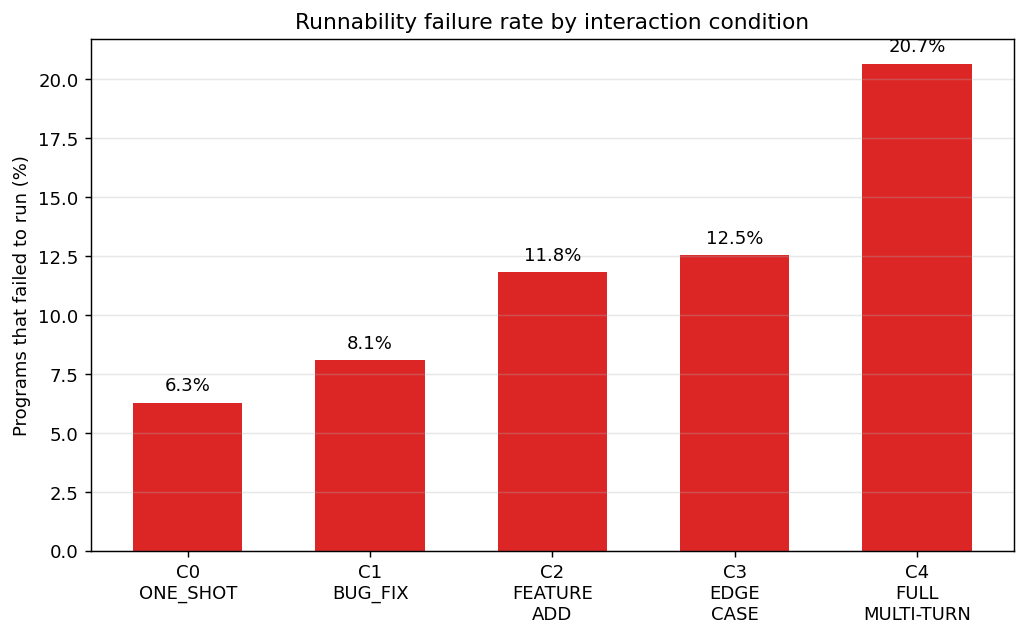
\includegraphics[width=\columnwidth]{images/fig11_failure_rate.png}
\caption{Genuine model-failure rate by condition (collection artifacts
excluded). Full multi-turn fails most
often---complexity has a correctness cost too.}
\label{fig:fail}
\end{figure}

\section{Discussion}
Multi-turn interaction leaves a measurable green-software footprint: the
median barely moves for single steps, but the full trajectory shifts the
median up and thickens the upper tail---most sessions cost little extra, a
minority cost a lot. Three mechanisms: (i) accumulated requirements produce
longer, less pruned code (+58 mean / +35 median SLOC C0$\rightarrow$C4);
(ii) feature/edge turns add defensive branches and extra input passes
(cyclomatic 13$\rightarrow$18); (iii) some trajectories converge on
asymptotically heavier solutions (C4 reliable-slope superlinear rate 18\%).

Static complexity rises with depth but correlates weakly with energy; the
mediator is runtime (energy $\approx$ power $\times$ time). Practitioners
should treat iterative features as potential complexity regressions and
re-benchmark the final artifact, demand asymptotic justification per turn,
and close long sessions with a complexity review. Tool builders should
surface per-turn complexity and energy deltas in the IDE---e.g.\ flagging a
turn that moves the estimate from $O(n\log n)$ to $O(n^2)$.

\section{Threats to Validity}\index{threats to validity}
\emph{Construct:} RAPL includes off-target components; identical workloads
and per-run baselines mitigate noise, and the estimator is cross-checked both
ways. \emph{Internal:} deterministic shared workloads and paired tests
control task difficulty; 111 genuine model failures bias coverage toward runnable
programs. \emph{External:} one host, Python only, four models.
\emph{Conclusion:} only C4 is
significant---single-step claims are withheld; the probe covers the
algorithms category while static metrics cover all 1418.

\section{Conclusion}
Holding final specification constant, full multi-turn trajectories increase
median package energy over one-shot generation (the only significant effect),
mediated by runtime and algorithm choice rather than source size alone. We
release a per-program corpus with dual static/empirical complexity estimates
and full reproduction scripts. Future work: more models, languages, and
hardware; per-turn energy attribution; automatic complexity-regression
detection; full-category scaling sweeps.

\section*{Acknowledgment}
Compute and measurement host providers; maintainers of Intel RAPL tooling.
[Add funding/grant acknowledgments before submission.]

\begin{thebibliography}{00}
\bibitem{rotem2012} E.~Rotem et al., ``Power-management architecture of the
Intel microarchitecture code-named Sandy Bridge,'' \emph{IEEE Micro},
vol.~32, no.~2, pp.~20--27, 2012.
\bibitem{hahnell2012} M.~H\"ahn et al., ``Measuring energy consumption for
short code paths using RAPL,'' \emph{ACM SIGMETRICS PER}, vol.~40, no.~3,
pp.~13--17, 2012.
\bibitem{hackenberg2013} D.~Hackenberg et al., ``An energy efficiency feature
survey of the Intel Haswell processor,'' in \emph{Proc.\ IPDPSW}, 2013.
\bibitem{schwartz2020} R.~Schwartz et al., ``Green AI,'' \emph{Commun.\ ACM},
vol.~63, no.~12, pp.~54--63, 2020.
\bibitem{patterson2021} D.~Patterson et al., ``Carbon emissions and large
neural network training,'' arXiv:2104.10350, 2021.
\bibitem{strubell2019} E.~Strubell et al., ``Energy and policy considerations
for deep learning in NLP,'' in \emph{Proc.\ ACL}, 2019.
\bibitem{georgiou2022} S.~Georgiou et al., ``Green AI: Do deep learning
frameworks have different costs?'' \emph{Empir.\ Softw.\ Eng.}, vol.~27,
2022.
\bibitem{hindle2023} A.~Hindle, ``Green software engineering: The curse of
methodology,'' \emph{Empir.\ Softw.\ Eng.}, 2023.
\bibitem{pinto2014} G.~Pinto et al., ``Understanding energy behaviors of
thread management constructs,'' in \emph{Proc.\ OOPSLA}, 2014.
\bibitem{pereira2017} R.~Pereira et al., ``Energy efficiency across
programming languages,'' in \emph{Proc.\ SLE}, 2017.
\bibitem{chen2021} M.~Chen et al., ``Evaluating large language models trained
on code,'' arXiv:2107.03374, 2021.
\bibitem{austin2021} J.~Austin et al., ``Program synthesis with large language
models,'' arXiv:2108.07732, 2021.
\bibitem{nijkamp2023} R.~Nijkamp et al., ``CodeGen: An open large language
model for code with multi-turn program synthesis,'' in \emph{Proc.\ ICLR},
2023.
\bibitem{mccabe1976} T.~McCabe, ``A complexity measure,'' \emph{IEEE Trans.\
Softw.\ Eng.}, vol.~SE-2, no.~4, pp.~308--320, 1976.
\bibitem{pinto2014b} G.~Pinto et al., ``Energy efficiency: A new concern for
software engineers,'' in \emph{Proc.\ SAC}, 2014.
\bibitem{codecarbon2021} J.~Schmidt et al., ``CodeCarbon: Estimate and track
carbon emissions from ML computing,'' GitHub, 2021.
\bibitem{hotcarbon2022} A.~Anwar et al., ``Datacenter-scale energy and carbon
accounting,'' in \emph{Proc.\ HotCarbon}, 2022.
\bibitem{jimenez2024} C.~E.~Jimenez et al., ``SWE-bench: Can language models
resolve real-world GitHub issues?'' in \emph{Proc.\ ICLR}, 2024.
\bibitem{sweagent2024} J.~Yang et al., ``SWE-agent: Agent--computer interfaces
enable automated software engineering,'' in \emph{Proc.\ NeurIPS}, 2024.
\bibitem{codellama2023} B.~Rozi\`ere et al., ``Code Llama: Open foundation
models for code,'' arXiv:2308.12950, 2023.
\bibitem{deepseek2024} D.~Guo et al., ``DeepSeek-Coder: When the large
language model meets programming,'' arXiv:2401.14196, 2024.
\bibitem{claude2024} Anthropic, ``Claude 3.5 Sonnet model card,'' 2024.
\bibitem{gemini2024} Google DeepMind, ``Gemini 1.5 model card,'' 2024.
\bibitem{gpt4o2024} OpenAI, ``GPT-4o system card,'' 2024.
\end{thebibliography}

\printindex

\end{document}
